\documentclass{beamer}
\usetheme{tokitex}

\usepackage{tikz}
\usepackage{graphics}
\usepackage{multirow}
\usepackage{tabto}

\usepackage[english,bahasa]{babel}
\newtranslation[to=bahasa]{Section}{Bagian}
\newtranslation[to=bahasa]{Subsection}{Subbagian}

\usepackage{listings, lstautogobble}
\usepackage{color}

\definecolor{dkgreen}{rgb}{0,0.6,0}
\definecolor{gray}{rgb}{0.5,0.5,0.5}
\definecolor{mauve}{rgb}{0.58,0,0.82}

\lstset{frame=tb,
  language=c++,
  aboveskip=1mm,
  belowskip=1mm,
  showstringspaces=false,
  columns=fullflexible,
  keepspaces=true,
  basicstyle={\small\ttfamily},
  numbers=none,
  numberstyle=\tiny\color{gray},
  keywordstyle=\color{blue},
  commentstyle=\color{dkgreen},
  stringstyle=\color{mauve},
  breaklines=true,
  breakatwhitespace=true,
  autogobble=true
}

\usepackage{caption}
\captionsetup[figure]{labelformat=empty}

\newcommand{\progTerm}[1]{\texttt{#1}}
\newcommand{\foreignTerm}[1]{\textit{#1}}
\newcommand{\newTerm}[1]{\alert{\textbf{#1}}}
\newcommand{\emp}[1]{\alert{#1}}
\newcommand{\statement}[1]{"#1"}


\title{Ekspresi}
\author{Tim Olimpiade Komputer Indonesia}
\date{}

\begin{document}

\begin{frame}
\titlepage
\end{frame}

\begin{frame}[fragile]
\frametitle{Kilas Balik: Assignment}
\begin{itemize}
  \item Program menjadi kurang bermanfaat jika kita hanya bisa mengisi variabel dengan nilai yang pasti. 
  \item Kadang-kadang dibutuhkan hal yang lebih ekspresif seperti penjumlahan:
\begin{lstlisting}
a = 5;
b = 2;
jumlah = a + b;
\end{lstlisting}
  \item Kenyataannya, hal ini dapat diwujudkan pada pemrograman.
  \item Perintah "a + b" biasa disebut sebagai \alert{ekspresi}.
\end{itemize}
\end{frame}

\begin{frame}
\frametitle{Mengenal Ekspresi}
\begin{figure}
  \centering
  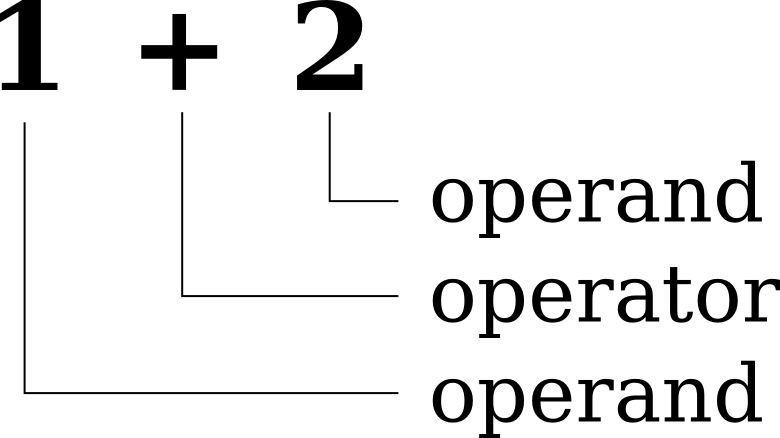
\includegraphics[width=4 cm]{asset/ekspresi.png}
\end{figure}
\begin{itemize}
  \item Ekspresi terdiri dari dua komponen: \alert{operator} dan \alert{operand}.
  \item Operand menyatakan nilai yang akan dioperasikan, misalnya bilangan atau suatu ekspresi lagi.
  \item Operator menyatakan bagaimana operand akan dioperasikan, apakah ditambah, dikali, atau dibagi?
\end{itemize}
\end{frame}

\begin{frame}
\frametitle{Mengenal Ekspresi (lanj.)}
Bisa juga dibentuk ekspresi bersarang, yaitu ekspresi yang operand-nya merupakan ekspresi lagi:
\begin{figure}
  \centering
  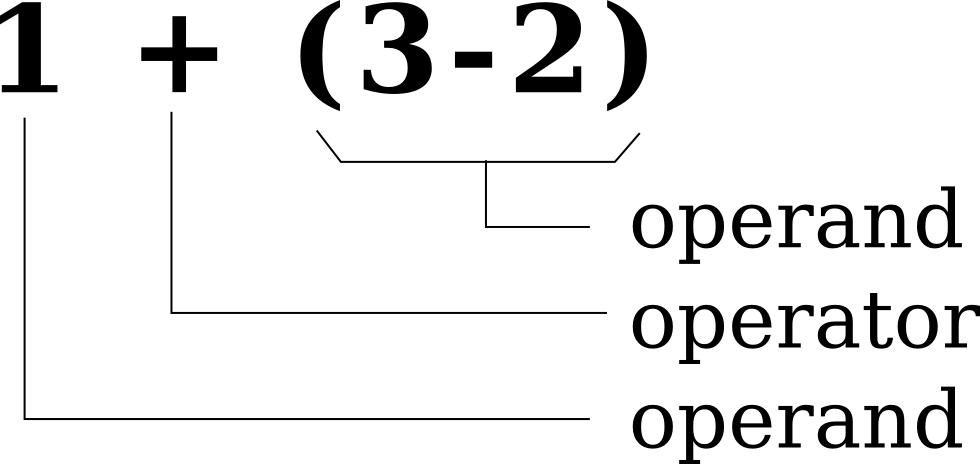
\includegraphics[width=5 cm]{asset/ekspresi-nested.png}
\end{figure}
\end{frame}

\begin{frame}
\frametitle{Operasi Numerik}
\begin{itemize}
  \item Operasi pada bilangan yang dapat dilakukan adalah penjumlahan (+), pengurangan (-), perkalian (*), pembagian (/), dan modulo (\%).
  \item Jika kedua operand merupakan bilangan bulat, hasil pengoperasian selalu bilangan bulat juga.
  \item Ketika setidaknya salah satu dari operand ada yang bertipe data \textit{floating point}, pengoperasian akan selalu menghasilkan \textit{floating point}.
\end{itemize}
\end{frame}

\begin{frame}
\frametitle{Operasi Numerik (lanj.)}
\begin{itemize}
  \item Operasi pembagian pada kedua operand berupa bilangan bulat didefinisikan sebagai: membagi, lalu dibulatkan ke bawah. Contoh:
  \begin{itemize}
    \item 7 / 2 = 3
    \item 10 / 2 = 5
    \item 3 / 5 = 0
  \end{itemize}
  \item Operasi pembagian dengan salah satu operand berupa \textit{floating point} akan menghasilkan \textit{floating point} pula. Contoh:
    \begin{itemize}
      \item 10.0 / 5 = 2.0000000
      \item 7 / 2.0 = 3.5000000
    \end{itemize}
\end{itemize}
\end{frame}

\begin{frame}
\frametitle{Operasi Numerik (lanj.)}
\begin{itemize}
  \item Operasi modulo adalah mengambil sisa bagi dari operand pertama terhadap operand kedua. Contoh:
  \begin{itemize}
    \item 7 mod 2 = 1
    \item 10 mod 2 = 0
    \item 3 mod 5 = 3
    \item 8 mod 3 = 2
  \end{itemize}
  \item Operasi mod hanya bisa dilakukan apabila kedua operand memiliki tipe data \alert{bilangan bulat}.
\end{itemize}
\end{frame}


\begin{frame}[fragile]
\frametitle{Contoh Program: kuadrat.cpp}
\begin{itemize}
  \item Setelah memahami tentang operasi numerik, coba perhatikan program berikut dan cari tahu apa keluarannya!
\begin{lstlisting}
#include <cstdio>

int a, b, c, x, hasil;

int main() {
  a = 1;
  b = 3;
  c = -2;
  x = 2;

  hasil = a*x*x + b*x + c;
  printf("ax^2 + bx + c = %d\n", hasil);
}\end{lstlisting}
\end{itemize}
\end{frame}

\begin{frame}
\frametitle{Prioritas Pengerjaan}
\begin{itemize}
  \item Seperti pada ilmu matematika, ada juga prioritas pengerjaan pada ekspresi numerik. Tabel berikut menunjukkan prioritasnya:

  \begin{tabular}{|c|c|}
  \hline Prioritas & Operasi \\
  \hline 1 & *,/,mod \\
  \hline 2 & +,- \\
  \hline
  \end{tabular}
  \item Jika ada beberapa operasi bersebelahan yang memiliki prioritas sama, operasi yang terletak di posisi lebih kiri akan dikerjakan lebih dahulu.
\end{itemize}
\end{frame}

\begin{frame}[fragile]
\frametitle{Contoh Program: numerik.cpp}
\begin{itemize}
  \item Kita juga bisa menggunakan tanda kurung untuk mengatur prioritas pengerjaan suatu ekspresi.
  \item Perhatikan contoh berikut dan coba jalankan programnya:
\begin{lstlisting}
#include <cstdio>

int hasil1, hasil2;

int main() {
  hasil1 = 3+5 / 4;
  hasil2 = (3+5) / 4;
  printf("%d\n", hasil1);
  printf("%d\n", hasil2);
}
\end{lstlisting}
  \item Isi dari variabel hasil1 adalah 4, karena operasi "5 div 4" memiliki prioritas yang lebih tinggi untuk dikerjakan, dan menghasilkan nilai 1. Barulah "3 + 1" dilaksanakan.
\end{itemize}
\end{frame}

\begin{frame}
\frametitle{Operasi Unary}
\begin{itemize}
  \item Pada C++, terdapat pula operasi \foreignTerm{unary} numerik.
  \item Operasi \foreignTerm{unary} berarti hanya melibatkan satu operand.
  \item Misalnya terdapat variabel \texttt{x}, operasi \foreignTerm{unary} tersedia berupa:
  \begin{itemize}
    \item \texttt{x++}, artinya tambah \texttt{x} dengan 1.
    \item \texttt{x--}, artinya kurangi \texttt{x} dengan 1.
  \end{itemize}
\end{itemize}
\end{frame}

\begin{frame}[fragile]
\frametitle{Contoh Operasi Unary}
Perhatikan dan coba eksekusi program berikut untuk memahami operasi \foreignTerm{unary}:
\begin{lstlisting}
#include <cstdio>

int main() {
  int x = 5;

  x++;
  printf("x: %d\n", x);

  x--;
  printf("x: %d\n", x);
}
\end{lstlisting}
\end{frame}

\begin{frame}
\frametitle{Fungsi Dasar Numerik}
Untuk membantu perhitungan, C++ menyediakan fungsi-fungsi pada STL "cmath".
\begin{itemize}
  \item \texttt{round}: membulatkan suatu bilangan pecahan bilangan bulat terdekat (hasilnya tetap bertipe \foreignTerm{floating point}). Contoh: \texttt{round(1.2)} akan menghasilkan 1.0, sementara \texttt{round(1.87)} akan menghasilkan 2.0.
  \item \texttt{sqrt}: mendapatkan akar kuadrat dari suatu bilangan. Contoh: \texttt{sqrt(9)} akan menghasilkan 3.00, dan \texttt{sqrt(3)} akan menghasilkan 1.73205....
\end{itemize}
\end{frame}

\begin{frame}[fragile]
\frametitle{Contoh Program: cmath.cpp}
\begin{itemize}
  \item Perhatikan contoh penggunaan STL cmath berikut:
\begin{lstlisting}
#include <cstdio>
#include <cmath>

int main() {
  printf("%lf\n", sqrt(5));
  printf("%lf\n", round(5.2));
  printf("%lf\n", round(5.6));
}
\end{lstlisting}
\end{itemize}
\end{frame}

\begin{frame}
\frametitle{Operasi Relasional}
\begin{itemize}
  \item Kita juga bisa melakukan operasi relasional, yaitu:
  \begin{itemize}
    \item kurang dari ($<$)
    \item lebih dari ($>$)
    \item sama dengan ($==$)
    \item kurang dari atau sama dengan ($<=$)
    \item lebih dari atau sama dengan ($>=$)
    \item tidak sama dengan ($!=$)
  \end{itemize}
  \item Operasi relasional harus melibatkan dua operand (ingat bahwa operand bisa jadi berupa ekspresi lagi), dan menghasilkan sebuah nilai kebenaran.
  \item Pada C++, nilai kebenaran dinyatakan dengan tipe data \alert{\textbf{boolean}}.
\end{itemize}
\end{frame}

\begin{frame}[fragile]
\frametitle{Contoh Program: relasional.cpp}
\begin{itemize}
  \item Perhatikan contoh berikut dan coba jalankan programnya:
\begin{lstlisting}
#include <cstdio>

int main() {
  printf("%d\n", 2 > 1);
  printf("%d\n", 2 < 1);
  printf("%d\n", 2 == 1);
  printf("%d\n", 2 >= 1);
  printf("%d\n", 1 == 1);
  printf("%d\n", 1 != 1);
  printf("%d\n", 1 != 2);
}
\end{lstlisting}
\end{itemize}
\end{frame}

\begin{frame}[fragile]
\frametitle{Operasi Relasional pada Floating Point}
\begin{itemize}
  \item Karena komputer tidak dapat secara sempurna menyimpan nilai \textit{floating point}, Anda perlu hati-hati saat membandingkan dua bilangan riil.
  \item Ekspresi berikut mungkin saja bernilai \textbf{FALSE}:
  \begin{lstlisting}
  (0.1 + 0.2) == 0.3
  \end{lstlisting}
  \item Sebab 0.1 + 0.2 bisa saja bernilai \textbf{0.30000000000000001}
\end{itemize}
\end{frame}

\begin{frame}
\frametitle{Operasi Relasional pada Floating Point (lanj.)}
\begin{itemize}
  \item Untuk memeriksa kesamaan antara dua nilai \textit{floating point}, biasanya dilibatkan suatu nilai toleransi.
  \item Misalnya, kedua nilai dianggap sama apabila selisih mereka kurang dari $10^{-8}$.
\end{itemize}
\end{frame}

\begin{frame}
\frametitle{Operasi Relasional (lanj.)}
\begin{itemize}
  \item Operasi relasional dapat dilakukan pada setiap tipe data ordinal, sehingga bisa juga diterapkan pada \textbf{char}.
  \item Perbandingan karakter dilakukan dengan membandingkan kode ASCII mereka, sehingga menjadi seperti membandingkan angka biasa.
  \item Contoh:
  \begin{itemize}
    \item 'a' $<$ 'b' akan bernilai \textbf{TRUE}
    \item 'a' $>$ 'z' bernilai \textbf{FALSE}
    \item 'A' $<$ 'a' akan bernilai \textbf{TRUE}
  \end{itemize}
\end{itemize}
\end{frame}

\begin{frame}
\frametitle{Operasi Relasional (string)}
\begin{itemize}
  \item Lebih jauh lagi, \textbf{string} sebenarnya merupakan untaian \textbf{char}. Operasi relasional juga bisa diterapkan pada \textbf{string} (meskipun \textbf{string} bukan tipe data ordinal).
  \item C++ akan membandingkan karakter demi karakter dari kiri ke kanan. Begitu ditemukan ada perbedaan karakter, lebih kecil atau tidaknya suatu string ditentukan oleh karakter tersebut.
  \begin{itemize}
    \item Contohnya, "aa" $<$ "ab" akan bernilai \textbf{TRUE}.
  \end{itemize}
  \item Jika sampai salah satu string habis dan tidak ditemukan ada perbedaan karakter, maka stirng yang lebih pendek dianggap lebih kecil.
  \begin{itemize}
    \item Contohnya "a" $<$ "aa" bernilai \textbf{TRUE}.
  \end{itemize}
\end{itemize}
\end{frame}

\begin{frame}[fragile]
\frametitle{Contoh Program: relasional2.pas}
\begin{itemize}
  \item Perhatikan contoh berikut dan coba jalankan programnya:
\begin{lstlisting}
#include <cstdio>

int main() {
  printf("%d\n", 'a' > 'A');
  printf("%d\n", 'a' < 'A');
  printf("%d\n", 'a' >= 'A');
  printf("%d\n", 'a' == 'A');

  printf("%d\n", "a" < "aa");
  printf("%d\n", "abcb" > "abca");
  printf("%d\n", "abc" == "abc");
  printf("%d\n", "abc" <= "abc");
}
\end{lstlisting}
\end{itemize}
\end{frame}

\begin{frame}
\frametitle{Operasi Boolean}
\begin{itemize}
  \item Operasi \textbf{boolean} merupakan operasi yang hanya melibatkan nilai-nilai kebenaran. Terdiri atas: \textbf{not} (!), \textbf{and} ($\&\&$), \textbf{or} ($||$), \textbf{xor} ( $\widehat{}$ ).
  \item Operasi-operasi ini sesuai dengan sebuah cabang ilmu matematika yang bernama "aljabar boolean".
  \item Operasi \alert{not} merupakan operasi \textit{unary}. Gunanya untuk membalik nilai kebenaran.
  \item Tabel berikut menunjukkan efek dari penggunaan \textbf{not}, yang cara penulisannya dengan tanda seru (!) sebelum variabelnya.
  \begin{tabular}{|c|c|}
  \hline a & !a \\
  \hline TRUE & FALSE \\
  \hline FALSE & TRUE \\
  \hline
  \end{tabular}
\end{itemize}
\end{frame}

\begin{frame}
\frametitle{Operasi Boolean (lanj.)}
\begin{itemize}
  \item Operasi \textbf{boolean} yang lainnya merupakan operasi \textit{binary}, yang artinya melibatkan dua operand.
  \item Tabel berikut menunjukkan efek dari penggunaan operator-operator tersebut:
  \begin{tabular}{|c|c|c|c|c|}
  \hline a & b & a \&\& b & a $||$ b & a $\widehat{}$ b \\
  \hline TRUE & TRUE & TRUE & TRUE & FALSE \\
  \hline TRUE & FALSE & FALSE & TRUE & TRUE \\
  \hline FALSE & TRUE & FALSE & TRUE & TRUE\\
  \hline FALSE & FALSE & FALSE & FALSE & FALSE \\
  \hline
  \end{tabular}
\end{itemize}
\end{frame}

\begin{frame}
\frametitle{Operasi Boolean (lanj.)}
\begin{itemize}
  \item Prioritas pengerjaan dari operator \textbf{boolean} secara berurutan adalah: \textbf{not}, \textbf{and}, \textbf{or}, \textbf{xor}.
  \item Tanda kurung juga bisa digunakan untuk menentukan operasi mana yang perlu dijalankan terlebih dahulu. Bahkan sangat disarankan untuk selalu menggunakan tanda kurung untuk kejelasan.
\end{itemize}
\end{frame}

\begin{frame}[fragile]
\frametitle{Contoh Program: relasional3.pas}
\begin{itemize}
  \item Perhatikan contoh berikut dan coba jalankan programnya:
\begin{lstlisting}
#include <cstdio>

int main() {
  printf("%d\n", 2 > 1);
  printf("%d\n", !(2 > 1));
  printf("%d\n", (2 > 1) && (3 > 1));
  printf("%d\n", ((2 > 1) || (3 < 1)) && (1 == 1));
  printf("%d\n", (1 != 1) ^ !(1 != 1));
}\end{lstlisting}
  \item Perhatikan bahwa tanda kurung diperlukan dalam ekspresi "not (2 $>$ 1)". Dengan tanda kurung, "2 $>$ 1" akan dievaluasi terlebih dahulu, menghasilkan nilai \textbf{boolean}. Barulah operator \textbf{not} bisa mengolah nilai \textbf{boolean} tersebut.
\end{itemize}
\end{frame}

\begin{frame}
\frametitle{Selanjutnya...}
\begin{itemize}
  \item Kini kalian sudah mempelajari tentang variabel, ekspresi, dan masukan/keluaran.
  \item Artinya, sudah waktunya untuk menulis program-program sederhana.
\end{itemize}
\end{frame}

\end{document}
